\documentclass[tikz]{standalone}
\usetikzlibrary{arrows.meta,calc}

% ------------------------------------------------------------
% Ground
% ------------------------------------------------------------

% \gardenGround{xmin}{xmax}
\newcommand{\gardenGround}[2]{%
  % main soil
  \fill[brown!55!black] (#1,-0.8) rectangle (#2,0.02);

  % darker lower layer for depth
  \fill[brown!35!black]
    (#1,-0.7)
    .. controls (#1+1.5,-0.58) and (#2-1.5,-0.82) .. (#2,-0.64)
    -- (#2,-0.8) -- (#1,-0.8) -- cycle;

  % grass strip
  \fill[green!50!black] (#1,0.02) rectangle (#2,0.12);

  % grass blades
  \pgfmathsetmacro{\xmin}{#1}
  \pgfmathsetmacro{\xmax}{#2}
  \foreach \i in {0,...,75} {
    \pgfmathsetmacro{\x}{\xmin + \i*(\xmax-\xmin)/75}
    \ifnum\i>0
      \draw[green!45!black, line width=0.45pt] (\x-0.03,0.04) -- ++(-0.07,0.14);
    \fi
    \draw[green!55!black, line width=0.45pt] (\x+0.00,0.04) -- ++(-0.03,0.18);

    \ifnum\i<75
      \draw[green!40!black, line width=0.45pt] (\x+0.03,0.04) -- ++(0.02,0.13);
    \fi
  }

  % little stones in the soil
  \foreach \x/\y in {
    -0.15/-0.26, 0.28/-0.49, 0.83/-0.31, 1.47/-0.57,
    1.92/-0.24, 2.63/-0.41, 2.88/-0.22, 3.54/-0.52,
    4.21/-0.28, 4.67/-0.44, 5.39/-0.21, 5.94/-0.58,
    6.18/-0.34, 6.91/-0.47, 7.56/-0.25
  }{
    \fill[brown!25!black] (\x,\y) ellipse (0.08 and 0.04);
  }
}

% ------------------------------------------------------------
% Empty hole
% ------------------------------------------------------------

% \hole{x}{scale}
\newcommand{\hole}[2]{%
  \begin{scope}[shift={(#1,0.02)},scale=#2]
    % dark cavity below ground
    \fill[brown!80!black]
      (-0.34,0)
      .. controls (-0.30,-0.16) and (-0.18,-0.34) .. (0,-0.42)
      .. controls (0.18,-0.34) and (0.30,-0.16) .. (0.34,0)
      -- cycle;

    % opening of the hole, flush with the ground
    \fill[brown!30!black] (0,0) ellipse (0.38 and 0.09);

    % front rim only, so it looks embedded in the soil
    \draw[brown!90!black, line width=0.7pt]
      (-0.38,0) arc[start angle=180,end angle=360,x radius=0.38,y radius=0.09];

    % small piles of displaced soil
    \fill[brown!55!black] (-0.48,0.02) ellipse (0.08 and 0.035);
    \fill[brown!55!black] ( 0.46,0.015) ellipse (0.07 and 0.03);
  \end{scope}
}

% ------------------------------------------------------------
% Flowerpot
% ------------------------------------------------------------

% \flowerpot{x}{y}{scale}
\newcommand{\flowerpot}[3]{%
  \begin{scope}[shift={(#1,#2)},scale=#3]
    % pot body
    \fill[orange!75!brown] (-0.40,-0.1) -- (0.40,-0.1) -- (0.25,-0.82) -- (-0.25,-0.82) -- cycle;
    \draw[brown!55!black,line width=0.9pt] (-0.40,-0.1) -- (0.40,-0.1) -- (0.25,-0.82) -- (-0.25,-0.82) -- cycle;

    % rim
    \fill[orange!88!brown] (-0.5,-0.1) rectangle (0.50,0.1);
    \draw[brown!55!black,line width=0.9pt] (-0.50,-0.1) rectangle (0.50,0.1);
  \end{scope}
}

% \flowerpotwithflower{x}{y}{scale}{flower code}
\newcommand{\flowerpotwithflower}[4]{%
  \begin{scope}[shift={(#1,#2)},scale=#3]
    \begin{scope}[shift={(0,0.1)}]
      #4
    \end{scope}
    \flowerpot{0}{0}{1}
  \end{scope}
}

% ------------------------------------------------------------
% Stem tag
% ------------------------------------------------------------
% \stemtag{x}{y}{stemheight}{text}{side}
% side should be 1 for right, -1 for left
\newcommand{\stemtag}[5]{%
  \begin{scope}[shift={(#1,#2)}]
    % vertical placement of the tag along the stem
    \pgfmathsetmacro{\ty}{0.42*#3}
    \pgfmathsetmacro{\sx}{#5}

    % little strings tying the tag to the stem
    \draw[brown!60!black, line width=0.45pt]
      (0,\ty+0.03) .. controls (0.05*\sx,\ty+0.05) and (0.10*\sx,\ty+0.04) .. (0.17*\sx,\ty+0.02);
    \draw[brown!60!black, line width=0.45pt]
      (0,\ty-0.03) .. controls (0.05*\sx,\ty-0.05) and (0.10*\sx,\ty-0.04) .. (0.17*\sx,\ty-0.02);

    % tag body
    \fill[white, rounded corners=1.2pt]
      (0.17*\sx,\ty+0.2) rectangle (0.6*\sx,\ty-0.2);

    \draw[black!70, line width=0.5pt, rounded corners=1.2pt]
      (0.17*\sx,\ty+0.2) rectangle (0.6*\sx,\ty-0.2);

    % small hole in the tag
    \fill[black!50] (0.21*\sx,\ty) circle (0.02);

    % number/text written on the tag
    \node[font=\large] at (0.4*\sx,\ty) {#4};
  \end{scope}
}


\begin{document}

\begin{tikzpicture}[x=1cm,y=1cm]
  \path[use as bounding box] (-0.8,-0.9) rectangle (8.5,3);

  \gardenGround{-0.5}{8.3}

  \node[anchor=south] at (0.1,-0.6) {
    
\includegraphics[height=3cm]{hydrangea.png}
  };
  \stemtag{0.3}{0.12}{1.35}{3}{1}

  \node[anchor=south,xscale=-1] at (1.7,-0.3) {
    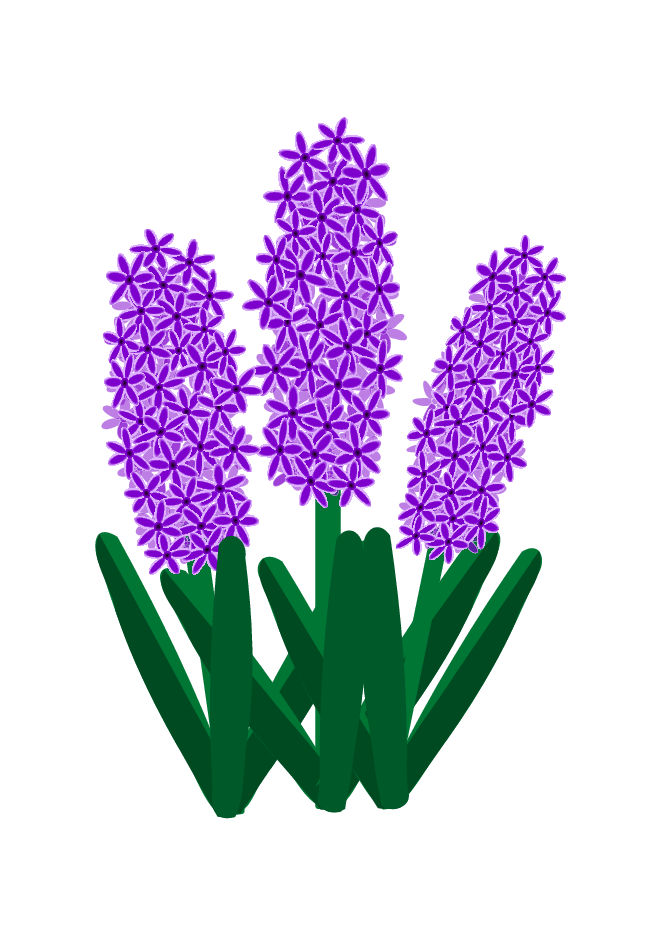
\includegraphics[height=2cm]{hyacinth.png}
  };
  \stemtag{1.7}{0.12}{1}{1}{-1}

  \node[anchor=south,xscale=-1] at (3.1,-0.6) {
    
\includegraphics[height=2.8cm]{hydrangea.png}
  };
  \stemtag{3.3}{0.12}{1.55}{3}{1}

  \node[anchor=south] at (4.9,-0.2) {
    
\includegraphics[scale=0.07]{tulip.pdf}
  };
  \stemtag{4.8}{0.12}{1.28}{5}{-1}

  \node[anchor=south] at (6.2,-0.3) {
    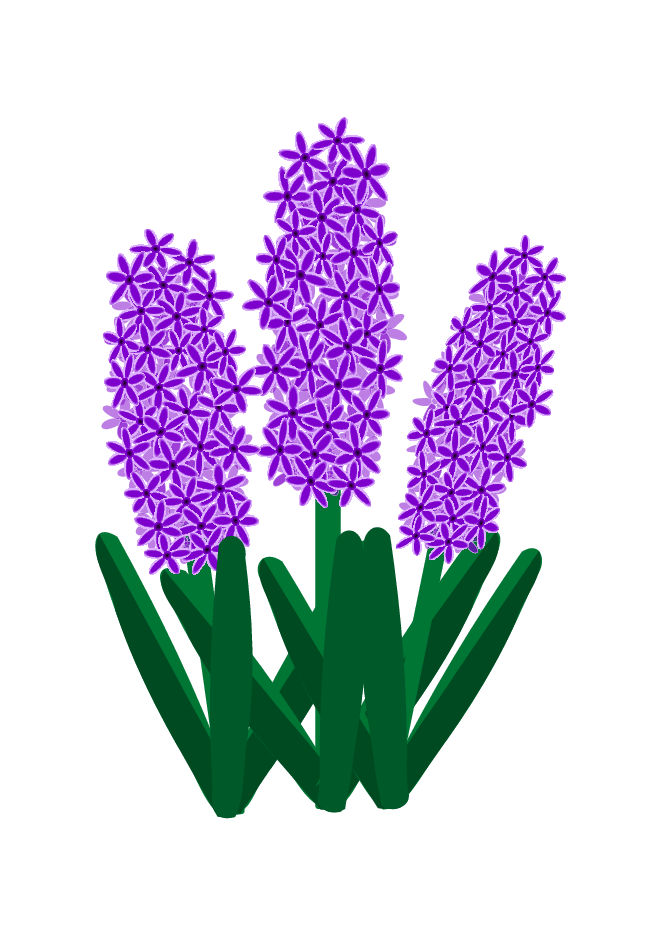
\includegraphics[height=2.2cm]{hyacinth.png}
  };
  \stemtag{6.2}{0.12}{1}{1}{-1}

  \flowerpotwithflower{7.8}{0.85}{1.0}{
  }

  \draw[-{Latex[length=3mm]},thick,blue!70!black]
    (4.8,1.8) to[bend left=60] (7.8,1.2);

\end{tikzpicture}

\end{document}
